\chapter{Installazione ed Esecuzione}
\lstset{basicstyle=\normalsize}
Nel presente capitolo verrà fornita una rapida guida d'installazione per l'utente e verrà illustrato un esempio di funzionamento dell'applicazione.
\section{Installazione}
Per generare il Makefile bisogna seguire i seguenti passi: 
\begin{enumerate}
\item Posizionarsi nella radice del progetto; 
\item Eseguire il file \lstinline{./autogen.sh};
\begin{figure}[H]
\begin{center}
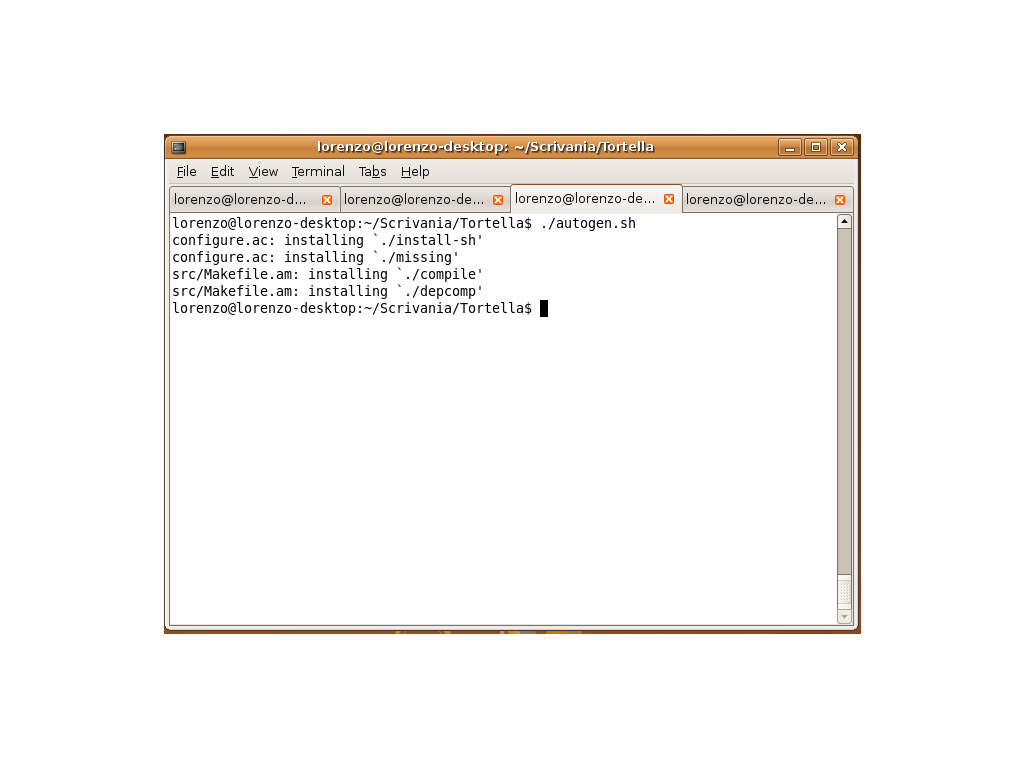
\includegraphics[scale=0.5]{etc/autogen.png}
\caption{autogen}
\label{autogen}
\end{center}
\end{figure}
\item Eseguire il \lstinline{./configure} sempre nella radice del progetto;
\begin{figure}[H]
\begin{center}
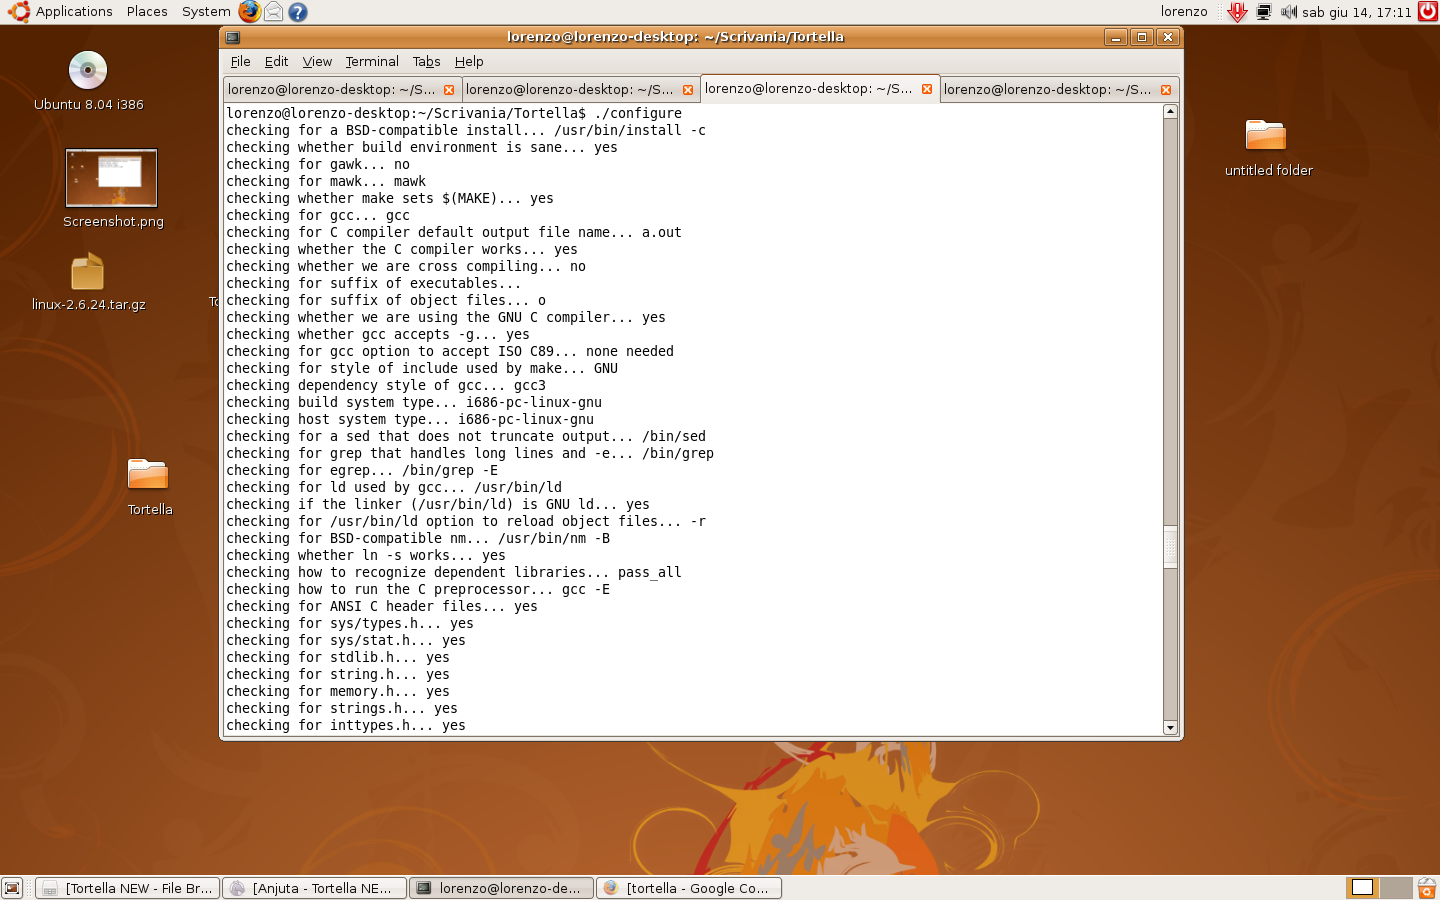
\includegraphics[scale=0.5]{etc/configure.png}
\caption{configure}
\label{configure}
\end{center}
\end{figure}
\item Ora il Makefile è pronto, per compilare basta eseguire \lstinline{make} dalla radice del progetto.
\begin{figure}[H]
\begin{center}
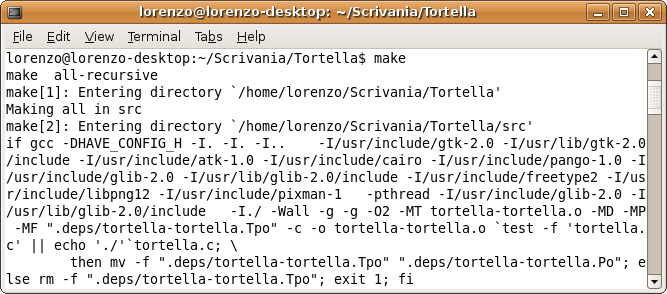
\includegraphics[scale=0.5]{etc/make.png}
\caption{make}
\label{make}
\end{center}
\end{figure}
\end{enumerate}
\section{Configurazione}
Prima di avviare il programma è necessario che i file vengano creati correttamente. A tal proposito si presenta un esempio di come dev'essere strutturato il file di configurazione e un esempio di come dev'essere strutturato il file contenente i "vicini" conosciuti:
\begin{lstlisting}
#TorTella Configuration file

#LOGGER
verbose = 3;

#SOCKET
qlen = 5;
buffer_len = 4096;

#PACKET
path = /tmp/tortella1;

#UTILS
gen_start = 100000;

#SERVENT
max_len = 4000;
max_thread = 20;
max_fd = 100;
timer_interval = 20;
new_connection_counter = 10000;

#SUPERNODE
datadir = ./data;

#SERVENT
local_ip = 127.0.0.1;
local_port = 2110;
nick = simo;
\end{lstlisting}
I primi due parametri sono relativi alla caratterizzazione del backlog massimo e della dimensione massima di un blocco di dati, di un socket di connessione. In particolare il parametro \texttt{qlen}\index{qlen} è utilizzato per impostare il numero massimo di  connessioni che possono essere gestite da un server, invece \texttt{buffer\_len} serve per imporre la dimensione massima del buffer che deve contenere una parte del pacchetto ricevuto. Tale frammento sarà poi concatenato con i restanti frammenti. La variabile \texttt{path}\index{path}, serve invece per memorizzare il percorso relativo in cui vengono salvati i log file, ampiamente utilizzato durante la fase di debugging e testing dell'intera applicazione. Il parametro \texttt{gen\_start}\index{gen\_start}, viene adottato nel meccanismo di identificazione univoco dell'utente, ovvero il valore impostato nel file serve come criterio di comparazione per la validazione del identificativo, associato all'utente stesso. In particolare distingue i fake ID con gli ID reali. Il parametro \texttt{timer\_interval}\index{timer\_interval} indica l'intervallo di tempo che il meccanismo di failure detection deve far passare tra i controlli. Il parametro \texttt{new\_connection\_counter}\index{new\_connection\_counter} indica il valore iniziale dei fake ID. Il parametro \texttt{verbose}\index{verbose} indica il livello di dettaglio delle stampe. Infine gli ultimi tre parametri sono necessari nella fase inizializzazione di ogni peer componente la rete, in quanto forniscono il relativo indirizzo ip, numero di porta del socket e nickname da assegnare all'utente.
Si consiglia all'utente inesperto di cambiare solamente gli ultimi tre parametri. Per quanto concerne il file di inizializzazione, questo dovrebbe essere strutturato in questo modo:
\begin{lstlisting}
127.0.0.1;2110;
127.0.0.1;2120;
\end{lstlisting}
Una volta che i file sono stati creati, è necessario posizionarli nelle directory corrette:
\begin{itemize}
\item Il file di esecuzione nella directory src;
\item file di configurazione in \lstinline{src/conf};
\item file di init in \lstinline{src/data}.
\end{itemize}
Se i file sono nelle posizioni corrette si può avviare l'esecuzione. Per l'esecuzione su una sola macchina è necessario avviare almeno due peer seguendo questi semplici passi:
\begin{enumerate}
\item Posizionarsi in src;
\item Eseguire \lstinline{./tortella ./conf/tortella.conf};
\item Eseguire \lstinline{./tortella ./conf/tortella1.conf ./data/init\_data}. 
\end{enumerate}
\section{Esecuzione}
L'esecuzione qui presentata viene eseguita su macchina locale simulando la presenza di tre peer nella rete. I tre peer, che per comodità verranno chiamati simo, lore, ibra saranno inizialmente connessi nel seguente modo: simo non conosce alcun peer vicino, lore e ibra invece conosceranno come unico vicino simo. I tre peer avviano l'applicazione e simo crea una chat dal nome "prova":
\begin{figure}[H]
\begin{center}
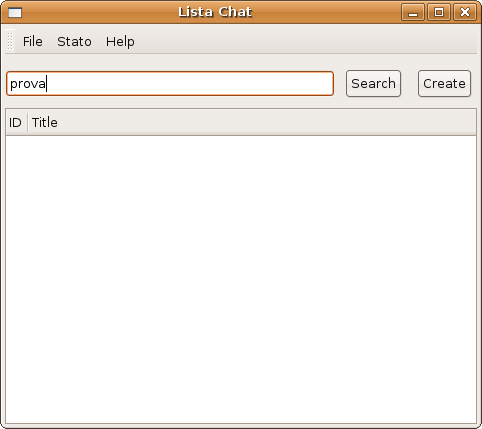
\includegraphics[scale=0.5]{etc/crea_chat.png}
\caption{Creazione della chat}
\label{creachat}
\end{center}
\end{figure}
\begin{figure}[H]
\begin{center}
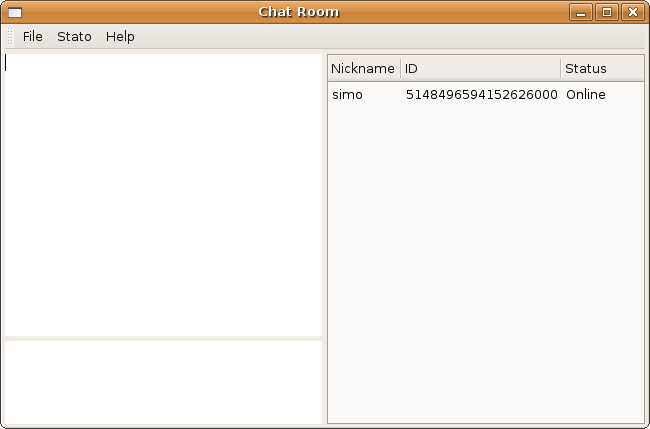
\includegraphics[scale=0.5]{etc/apertura_chat.png}
\caption{Apertura della chat}
\label{aperturachat}
\end{center}
\end{figure}
Lore cerca la chat "prova" e si connette:
\begin{figure}[H]
\begin{center}
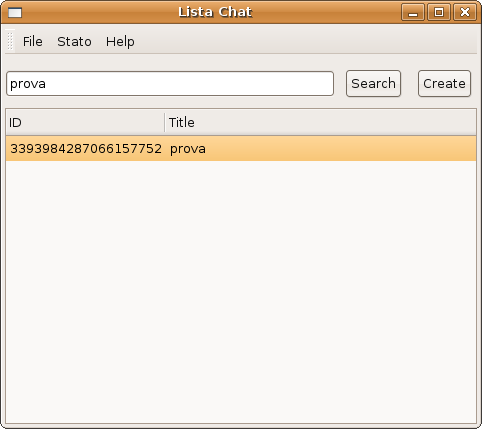
\includegraphics[scale=0.5]{etc/ricerca_lore.png}
\caption{Ricerca della chat}
\label{ricercalore}
\end{center}
\end{figure}
\begin{figure}[H]
\begin{center}
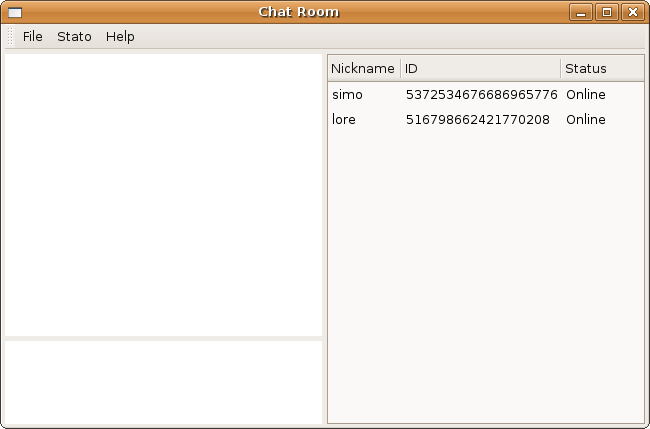
\includegraphics[scale=0.5]{etc/join_lore.png}
\caption{Join di lore}
\label{joinlore}
\end{center}
\end{figure}
ibra crea una chat di nome "pippo"
\begin{figure}[H]
\begin{center}
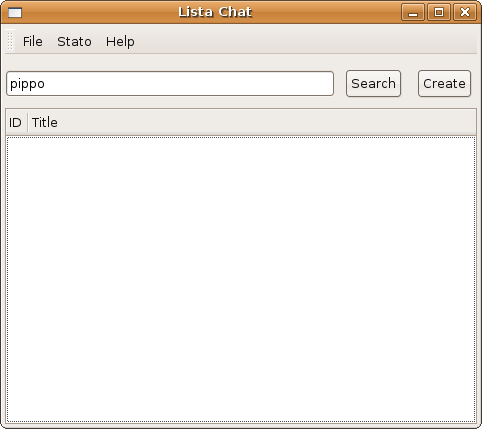
\includegraphics[scale=0.5]{etc/crea_chat2.png}
\caption{Creazione di una nuova chat}
\label{creachat2}
\end{center}
\end{figure}
Nell'attesa che qualcuno si connetta alla chat appena creata, ibra cerca la chat "prova" e si connette
\begin{figure}[H]
\begin{center}
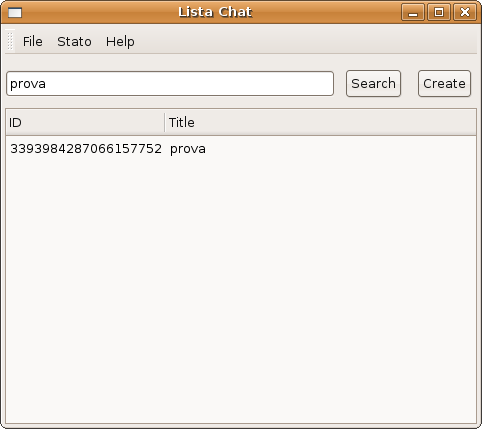
\includegraphics[scale=0.5]{etc/ricerca_chat_2.png}
\caption{Ricerca della chat prova}
\label{ricercachat2}
\end{center}
\end{figure}
\begin{figure}[H]
\begin{center}
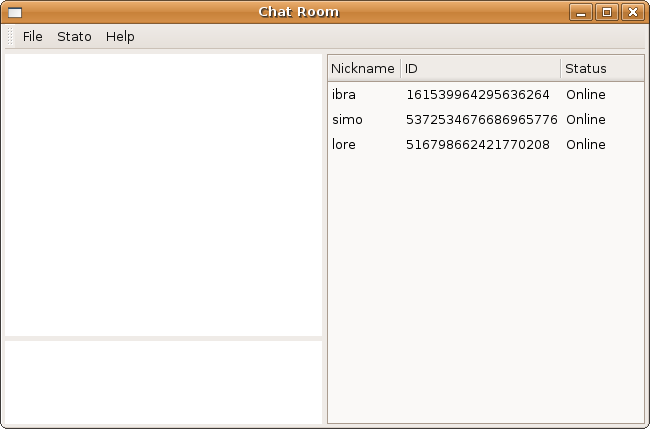
\includegraphics[scale=0.5]{etc/join2.png}
\caption{Join di ibra}
\label{join2}
\end{center}
\end{figure}
I tre utenti comunicano tra di loro
\begin{figure}[H]
\begin{center}
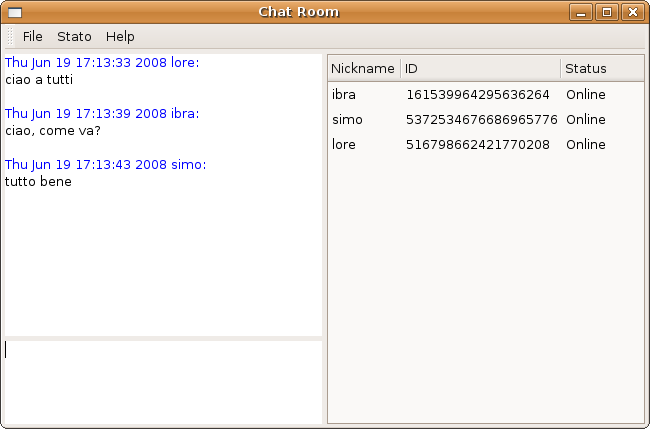
\includegraphics[scale=0.5]{etc/conversazione_chat.png}
\caption{Conversazione tra gli utenti}
\label{conversazionechat}
\end{center}
\end{figure}
lore invia un messaggio solo a simo (in realtà avrebbe potuto mandarlo a più utenti, ma essendo la chat composta da soli 3 utenti non avrebbe avuto senso mandare il messaggio a tutti)
\begin{figure}[H]
\begin{center}
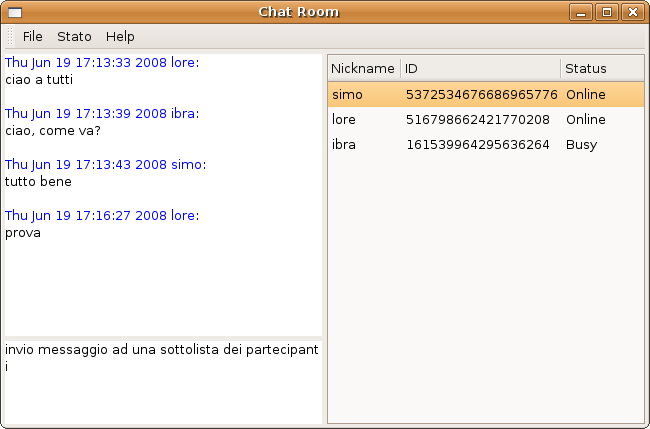
\includegraphics[scale=0.5]{etc/invio_sottolista.png}
\caption{Invio di un messaggio ad un sottoinsieme degli utenti}
\label{inviosottolista}
\end{center}
\end{figure}
lore invia un messaggio privato a ibra, che viene ricevuto correttamente da quest'ultimo
\begin{figure}[H]
\begin{center}
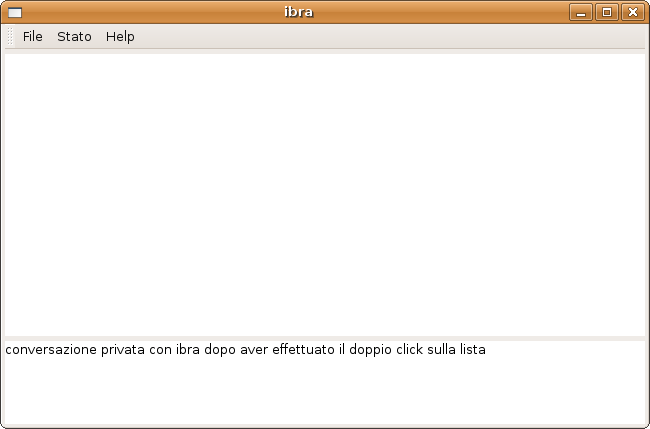
\includegraphics[scale=0.5]{etc/pm_ibra.png}
\caption{Invio di un messaggio privato}
\label{pmibra}
\end{center}
\end{figure}
\begin{figure}[H]
\begin{center}
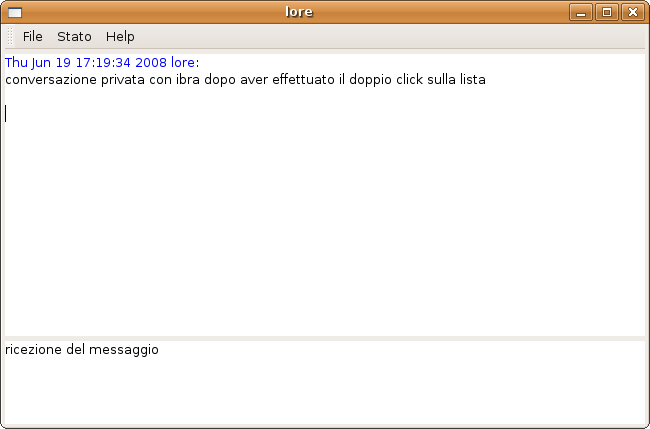
\includegraphics[scale=0.5]{etc/ricezione_pm.png}
\caption{Ricezione di un messaggio privato}
\label{ricezionepm}
\end{center}
\end{figure}
infine lore effettua il leave dalla chat e in seguito simo chiude l'applicazione inviando un bye ad ibra
\begin{figure}[H]
\begin{center}
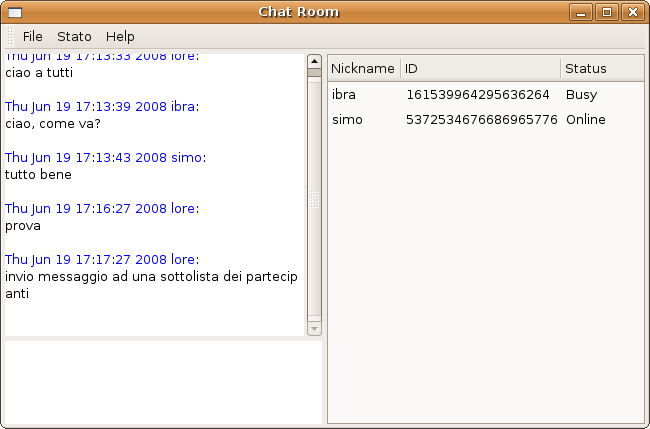
\includegraphics[scale=0.5]{etc/leave_lore.png}
\caption{Leave dalla chat prova}
\label{leavelore}
\end{center}
\end{figure}
\begin{figure}[H]
\begin{center}
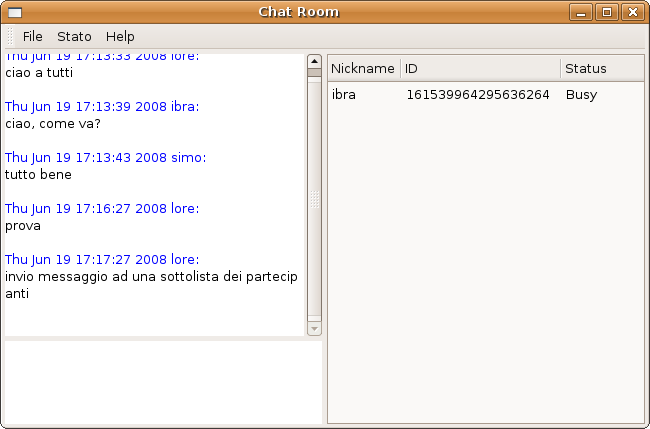
\includegraphics[scale=0.5]{etc/bye_simo.png}
\caption{Ricezione di un bye}
\label{byesimo}
\end{center}
\end{figure}
\lstset{basicstyle=\scriptsize}
